\section{Introduction}
%________________________________________
%CaRS Move I "Establish a territory" (Situation):
% * Important area
% * Introducing and reviewing items of previous  research <--(ToDO)

As humans, we often think in terms of cause and effect -- causality; if we understand why something happened, we can change our behavior to improve future outcomes. 
Causal inference is a process of determining the causality. The inference can be conducted in a controlled experiments, where the effect of one variable can be studied in isolation.
Some problems are however unsuitable for controlled experiments, where causal inference thus becomes more difficult. Determining the causality from real world data is such a problem, which can be difficult yet very important; for instance: to convincingly show that the emission of green house gases causes global warming, is perhaps the most important problem of our time. 

Data analysis can be used to show how variables vary together (correlation); however, correlation does not imply direct causality where: \emph{A} causes \emph{B} (\autoref{fig:direct_causation}). It could also be the opposite relation -- reversed causality (\autoref{fig:reversed_causation}). 
For instance: \emph{do windmills generate the wind, or is it the other way around?} There could also be a third hidden variable \emph{C}, causing both \emph{A} and \emph{B} -- common causality (\autoref{fig:common_causation}). For instance: \emph{if ice cream sales increase, the rate of drowning deaths also increases, so should you avoid ice cream when swimming?}
\begin{figure}[!htb]
    \begin{subfigure}[b]{0.3\textwidth}
        \centering
        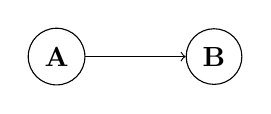
\begin{tikzpicture}[node distance=2cm]
        \node[circle,draw] at (0,0) (A) {\bf A};
        \node[circle,draw,right of=A] (B) {\bf B};
        \draw[->] (A) -- (B);
        \end{tikzpicture}
        \caption{Direct causality}
        \label{fig:direct_causation}
    \end{subfigure}
    \hfill
    \begin{subfigure}[b]{0.3\textwidth}
        \centering
        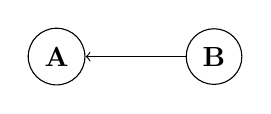
\begin{tikzpicture}[node distance=2cm]
        \node[circle,draw] at (0,0) (A) {\bf A};
        \node[circle,draw,right of=A] (B) {\bf B};
        \draw[<-] (A) -- (B);
        \end{tikzpicture}
        \caption{Reversed causality}
        \label{fig:reversed_causation}
    \end{subfigure}
    \hfill
    \begin{subfigure}[b]{0.3\textwidth}
        \centering
        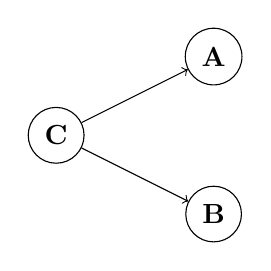
\begin{tikzpicture}[node distance=2cm]
        \node[circle,draw] at (0,0) (C) {\bf C};
        \node[circle,draw,right of=C,yshift=1cm] (A) {\bf A};
        \node[circle,draw,right of=C,yshift=-1cm] (B) {\bf B};
        \draw[->] (C) -- (A);
        \draw[->] (C) -- (B);
        \end{tikzpicture}
        \caption{Common causality}
        \label{fig:common_causation}
    \end{subfigure}
    \caption{Causality}
    \label{fig:causal_relationships}
    
\end{figure}

In ship hydrodynamics, experiments in a controlled laboratory environment with scale models (model tests) is a well established causal inference method.  
The model tests have some drawbacks such as: scale effects, and the fact that the laboratory environment as well as the test scenario are artificial idealizations of their real counterparts.
Data driven analysis on real ship operational data, instead of model tests, is a more direct way to analyze the ship's hydrodynamics, which has become more popular during the last years. The increased data collection onboard ships, as well as advancements within machine learning (ML), are probable drivers in this development. 

%________________________________________
%CaRS Move II "Establish a niche" (Problem):
% * counter claim?
% * gap?
% * question       <------
% * continuation? 
However, the real ship operational data is usually not collected from a controlled experiment, so that the causal inference thus becomes more challenging. Such a challenge is addressed in this paper: investigating a possible causal relationship between thrust allocation and fuel consumption of a double ended ferry -- Uraniborg (\autoref{fig:uraniborg}).
\begin{figure}[!htb]
    \centering
    \includegraphics[width=0.7\textwidth]{figures/GA_uraniborg.pdf}
    \caption{Double ended ferry Uraniborg, copyright Rederi AB Ventrafiken.}
    \label{fig:uraniborg}
\end{figure}
The thrust allocation concerns the load balance between the the ship's two azimuth thrusters: one in the aft, and one in the bow of the ship (\autoref{fig:uraniborg}). The two thrusters can run simultaneously, adding up to the total thrust force, driving the ship forward. The load balance can vary between all combinations from: full aft, to full forward thruster utilization (TU). This balance can be expressed with \autoref{eq:aft_thrust_ratio},
\begin{equation}
    TU = \frac{C_{aft}}{C_{aft} + C_{fwd}}
    \label{eq:aft_thrust_ratio}
\end{equation}
where $C_{aft}$ and $C_{fwd}$ are the fuel consumption from the aft and forward thruster.
\autoref{fig:fuel_consumption_correlation} shows data collected with a vessel monitoring system (https://online.blueflow.se/) from trips between Landskrona and Ven during one year for the variables: total fuel consumption, and $TU$. 
There seems to be a clear correlation between these variables,  which implies that there is relationship between them. But is it a direct causal relationship? Direct causality would mean that $TU$ can be used as an optimization parameter to reduce the fuel consumption.
\begin{figure}[!htb]
    \centering
    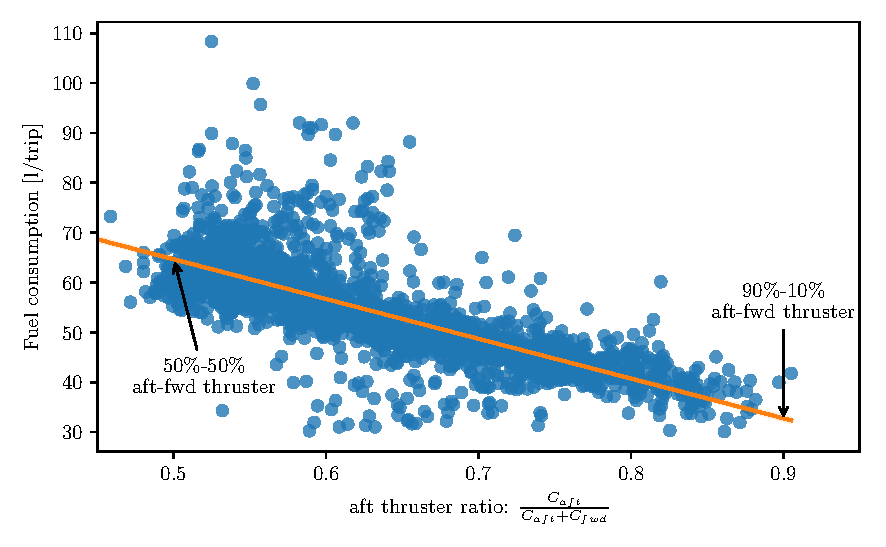
\includegraphics[width=\textwidth]{figures/correlation.pdf}
    \caption{Fuel consumption per trip with Uraniborg for trips during one year with varying aft thrust ratio.}
    \label{fig:fuel_consumption_correlation}
\end{figure}
However, both reversed causality or common causality are other possibilities, considering for instance these hypothetical scenarios:
\begin{itemize}
    \item Increased fuel consumption forces a reduced aft thruster utilization if the aft thruster is not strong enough. The forward thruster is then needed to add up to the higher power demand. (Reversed causality)

    \item There is a hidden variable such as bad weather which forces both thrusters to be used. (Common causality)
\end{itemize}
%________________________________________

%CaRS Move III "Occupy the niche" (Solution/Evaluation):
% * outline purpose?
% * list research questions?
% * announce principal findings?            <--
% * stating the value of present research?
% * article structure?                      <--
A controlled experiment was conducted onboard Uraniborg to infer the direct causal relationship. Results from this experiment are presented and analyzed in this paper to determine the relationship. Further, alternative methods applicable when the experiments cannot be conducted, are also investigated and discussed. It is investigated if the alternative methods can reach to the same conclusion as obtained from the controlled experiment inference.